\documentclass[draftcls,onecolumn]{IEEEtran}

%% INCLUDING THE PREAMBLE
%%%%%%%%%%%%%%%%%%%%%%%%%%%%%%%%%%%%%%%%%%%%%%%%%%%%%%%%%%%%%%%%%%%%%%%%%%%
%                                                                         %
%                                 PREAMBLE                                %
%                                                                         %
%%%%%%%%%%%%%%%%%%%%%%%%%%%%%%%%%%%%%%%%%%%%%%%%%%%%%%%%%%%%%%%%%%%%%%%%%%%

%% PACKAGES
\usepackage[]{lineno}
%\linenumbers
\usepackage[usenames,dvipsnames]{xcolor}
\usepackage{microtype}
\usepackage[obeyDraft]{todonotes}
\usepackage{fancyvrb}
\VerbatimFootnotes
\usepackage{algorithmic}

%% GRAPHICS RELATED
\usepackage{graphicx}
\usepackage[outdir=./tmp/]{epstopdf}
\graphicspath{{../images/}{./}{./tmp/}}
\DeclareGraphicsExtensions{.eps, .pdf, .jpeg, .png,}

%% CPATION SETUP
\usepackage{float}
\usepackage{caption}
\usepackage{subcaption}
\captionsetup{belowskip=12pt,aboveskip=4pt}


%% BIBLIOGRAPHY
\bibliographystyle{ieeetr}

%% UNITS
\usepackage{siunitx}

%% EQUATIONS
\usepackage{amsmath}
%\numberwithin{equation}{section}

%% HYPERLINKS
\usepackage[debug]{hyperref}

%%%%%%%%%%%%%%%%%%%%%%%%%%%%%%%%%%%%%%%%%%%%%%%%%%%%%%%%%%%%%%%%%%%%%%%%%%%
%                                                                         %
%                             Listing Setup                               %
%                                                                         %
%%%%%%%%%%%%%%%%%%%%%%%%%%%%%%%%%%%%%%%%%%%%%%%%%%%%%%%%%%%%%%%%%%%%%%%%%%%
\usepackage{listings}
\lstset{ %
    language=C++,
    basicstyle=\footnotesize\ttfamily,
    numbers=left,
    numberstyle=\tiny\color{gray},
    stepnumber=2,
    numbersep=5pt,
    backgroundcolor=\color{white},
    showspaces=false,
    showstringspaces=false,
    showtabs=false,
    frame=single,
    rulecolor=\color{black},
    tabsize=2,
    breaklines=true,
    breakatwhitespace=false,
    title=\lstname,
    keywordstyle=\color{blue},
    commentstyle=\color{OliveGreen},
    stringstyle=\color{orange}
}
\DeclareCaptionFont{white}{\color{white}}
\DeclareCaptionFormat{listing}{\colorbox[cmyk]{0.43, 0.35, 0.35, 0.01}{\parbox{\dimexpr\textwidth-2\fboxsep\relax}{#1#2#3}}}
\captionsetup[lstlisting]{format=listing,labelfont=white,textfont=white,singlelinecheck=false,margin=0pt,font={bf,footnotesize}}
%\lstnewenvironment{code}[1][]%
%{ \noindent\minipage{\linewidth}
%	\lstset{#1}
%}
%{\endminipage}
%% USER COMMANDS
\usepackage{isotope}
\newcommand{\iso}{\isotope}
\newcommand{\figurewidth}{\textwidth}
\newcommand{\micron}{$\mu$m}



%%%%%%%%%%%%%%%%%%%%%%%%%%%%%%%%%%%%%%%%%%%%%%%%%%%%%%%%%%%%%%%%%%%%%%%%%%%
%                                                                         %
%                                Start of Document                        %
%                                                                         %
%%%%%%%%%%%%%%%%%%%%%%%%%%%%%%%%%%%%%%%%%%%%%%%%%%%%%%%%%%%%%%%%%%%%%%%%%%%
\begin{document}
\title{Layered Detectors}
\author{Matthew J. Urffer}
\date{\today}
\maketitle


% Tables of Contents, Figures, Tables
\listoftodos
\tableofcontents
\listoffigures
\listoftables
\lstlistoflistings
%%%%%%%%%%%%%%%%%%%%%%%%%%%%%%%%%%%%%%%%%%%%%%%%%%%%%%%%%%%%%%%%%%%%%%%%%%%
%                                                                         %
%                              Start of Content                           %
%                                                                         %
%%%%%%%%%%%%%%%%%%%%%%%%%%%%%%%%%%%%%%%%%%%%%%%%%%%%%%%%%%%%%%%%%%%%%%%%%%%

\section{Introduction}
It has been observed that GS20 has a signficantly lower count rate per mass \iso[6]{Li} than other detectors measured at the Department of Nuclear Engineering Radiation Charaterization Labratories Neutron Irridiator.
It has been proposed by A. Mabe that the decrease in the count rate per mass \iso[6]{Li} could be explained by self-sheilding in the GS20 glass in which the large absorbtion cross section of the GS20 causes a depression of the flux within the detector volume.
The depression of flux within the detector volume then creates few neturon interactions and counts, which results in a lower count rate per mass absorber.
In order to determine if self-sheilding is responsible for this reducation a series of MCNPX calcuations are proposed in which the mass of the aborber is increased, as well as measuring the neutron flux in each cell.

\section{Methods}
MCNPX was used to simulate the neutron interactions for various mass fractions of \iso[6]{Li} in GS20 glass.
The cylindrical \SI{2}{\mm} thick detector was divided into 10 equal slices, each \SI{0.2}{\mm} thick.
In each cell the total number of $\iso[6]{Li}\left(\text{n},\text{t}\right)\alpha$ interactions was tallied by the use of a flux tally multiplied by the cross section, as well as tally the neutron flux.
This allows for the flux and reaction rate to plotted through the 
\begin{table}
  \centering
  \caption[GS20 Composition]{Comparison of GS20 Mass Fraction Compositions }
  \label{tab:GS20Comp}
  \begin{tabular}{c|c c c c c}
  \toprule
  & \ce{SiO2} & \ce{MgO} & \ce{Al2O3} & \ce{Li2O} \\
  \midrule
  Spowart (1976) & 57 & 4 & 18 & 4.0 & 17.1 \\
  AST & 56 & 4 & 18 & 4 & 18 \\
  \bottomrule
  \end{tabular}
\end{table}

The neutron flux in each cell was measured by taking \SI{0.2}{\mm} slices of the cylinderical \SI{2}{\mm} GS20 detector.
Thus, the each simulated flux has a surface contribution to it\footnote{assuming an isotropic impingnet neutron source, which after moderation is not unreasonable}, and is not a purecenter of material flux measurment.

\section{Results}
\begin{figure}
	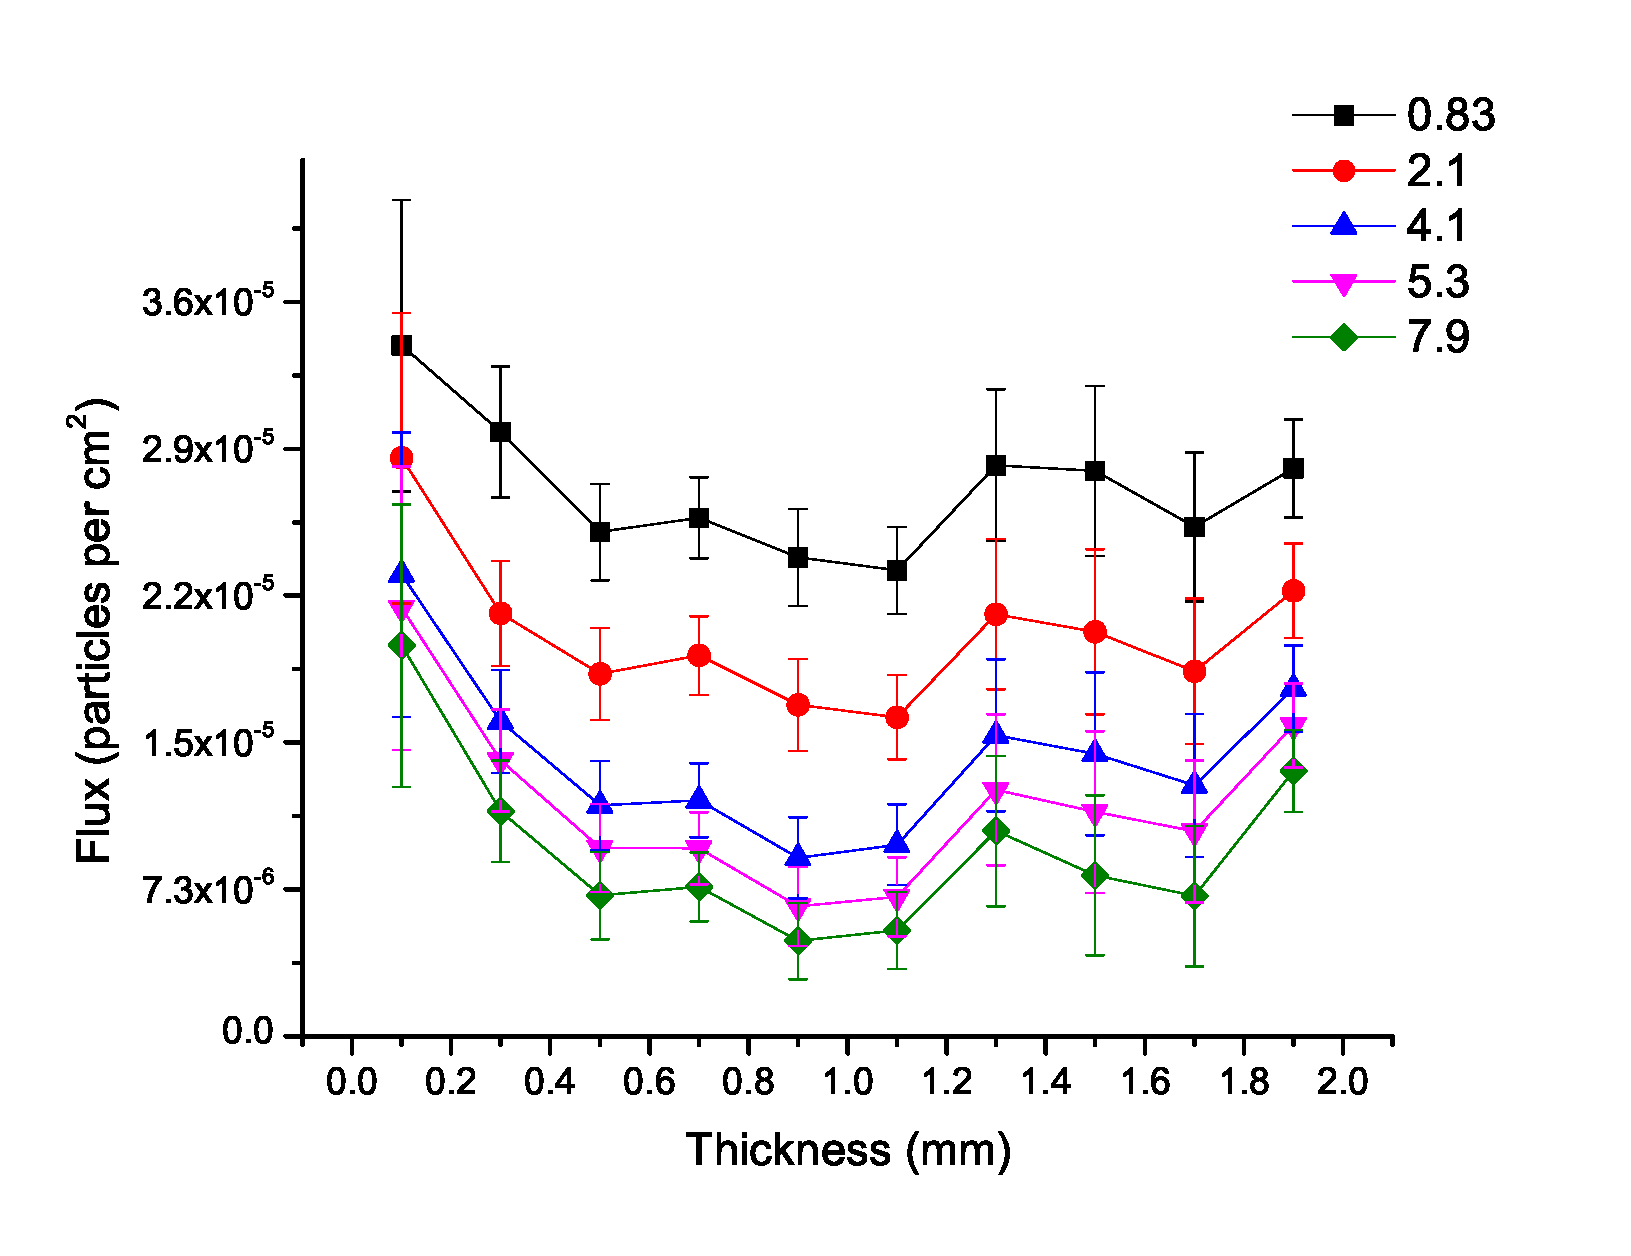
\includegraphics[width=\textwidth]{GS20SelfSheildFlux}
	\caption[Flux Profile through GS20]{}
	\labeli{fig:Flux}
\end{figure}
\begin{figure}
	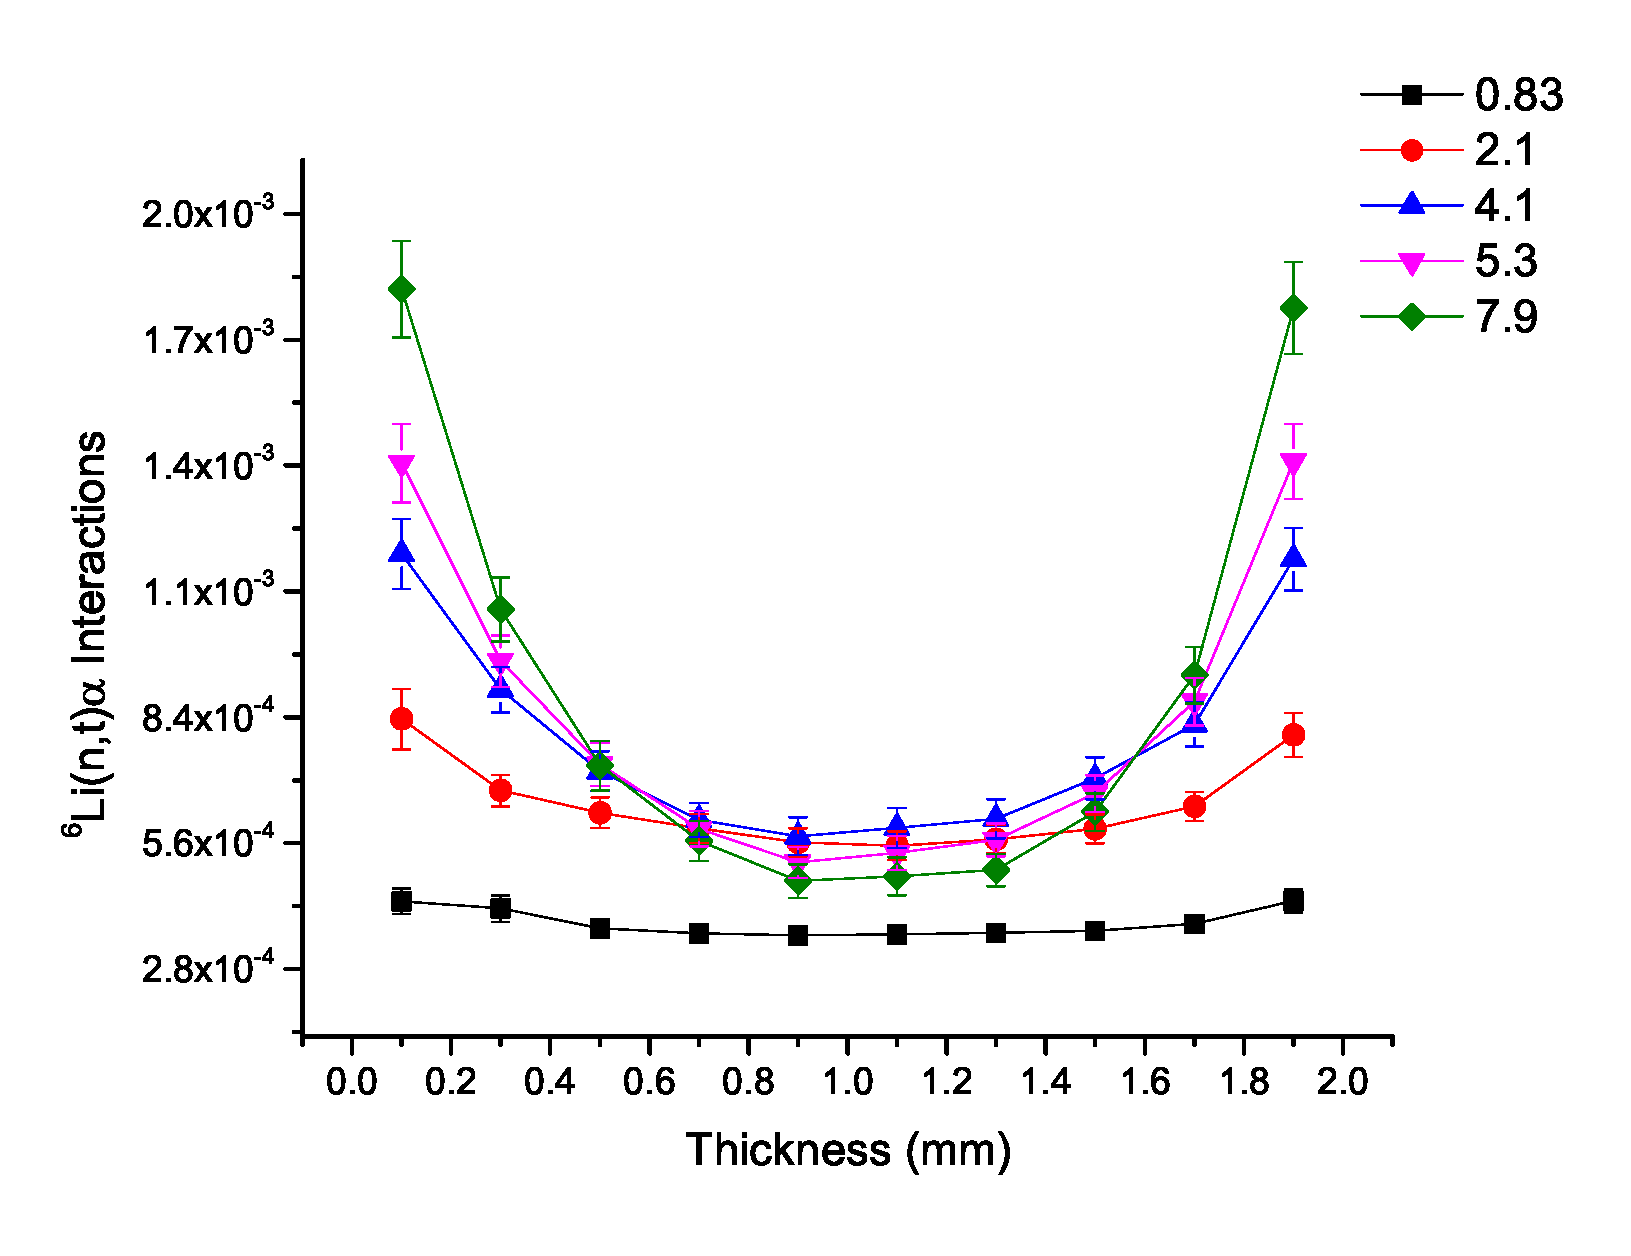
\includegraphics[width=\textwidth]{GS20SelfSheildRXNRate}
	\caption[Reaction Rate through GS20]{}
	\label{fig:RxnRate}
\end{figure}
\begin{figure}
	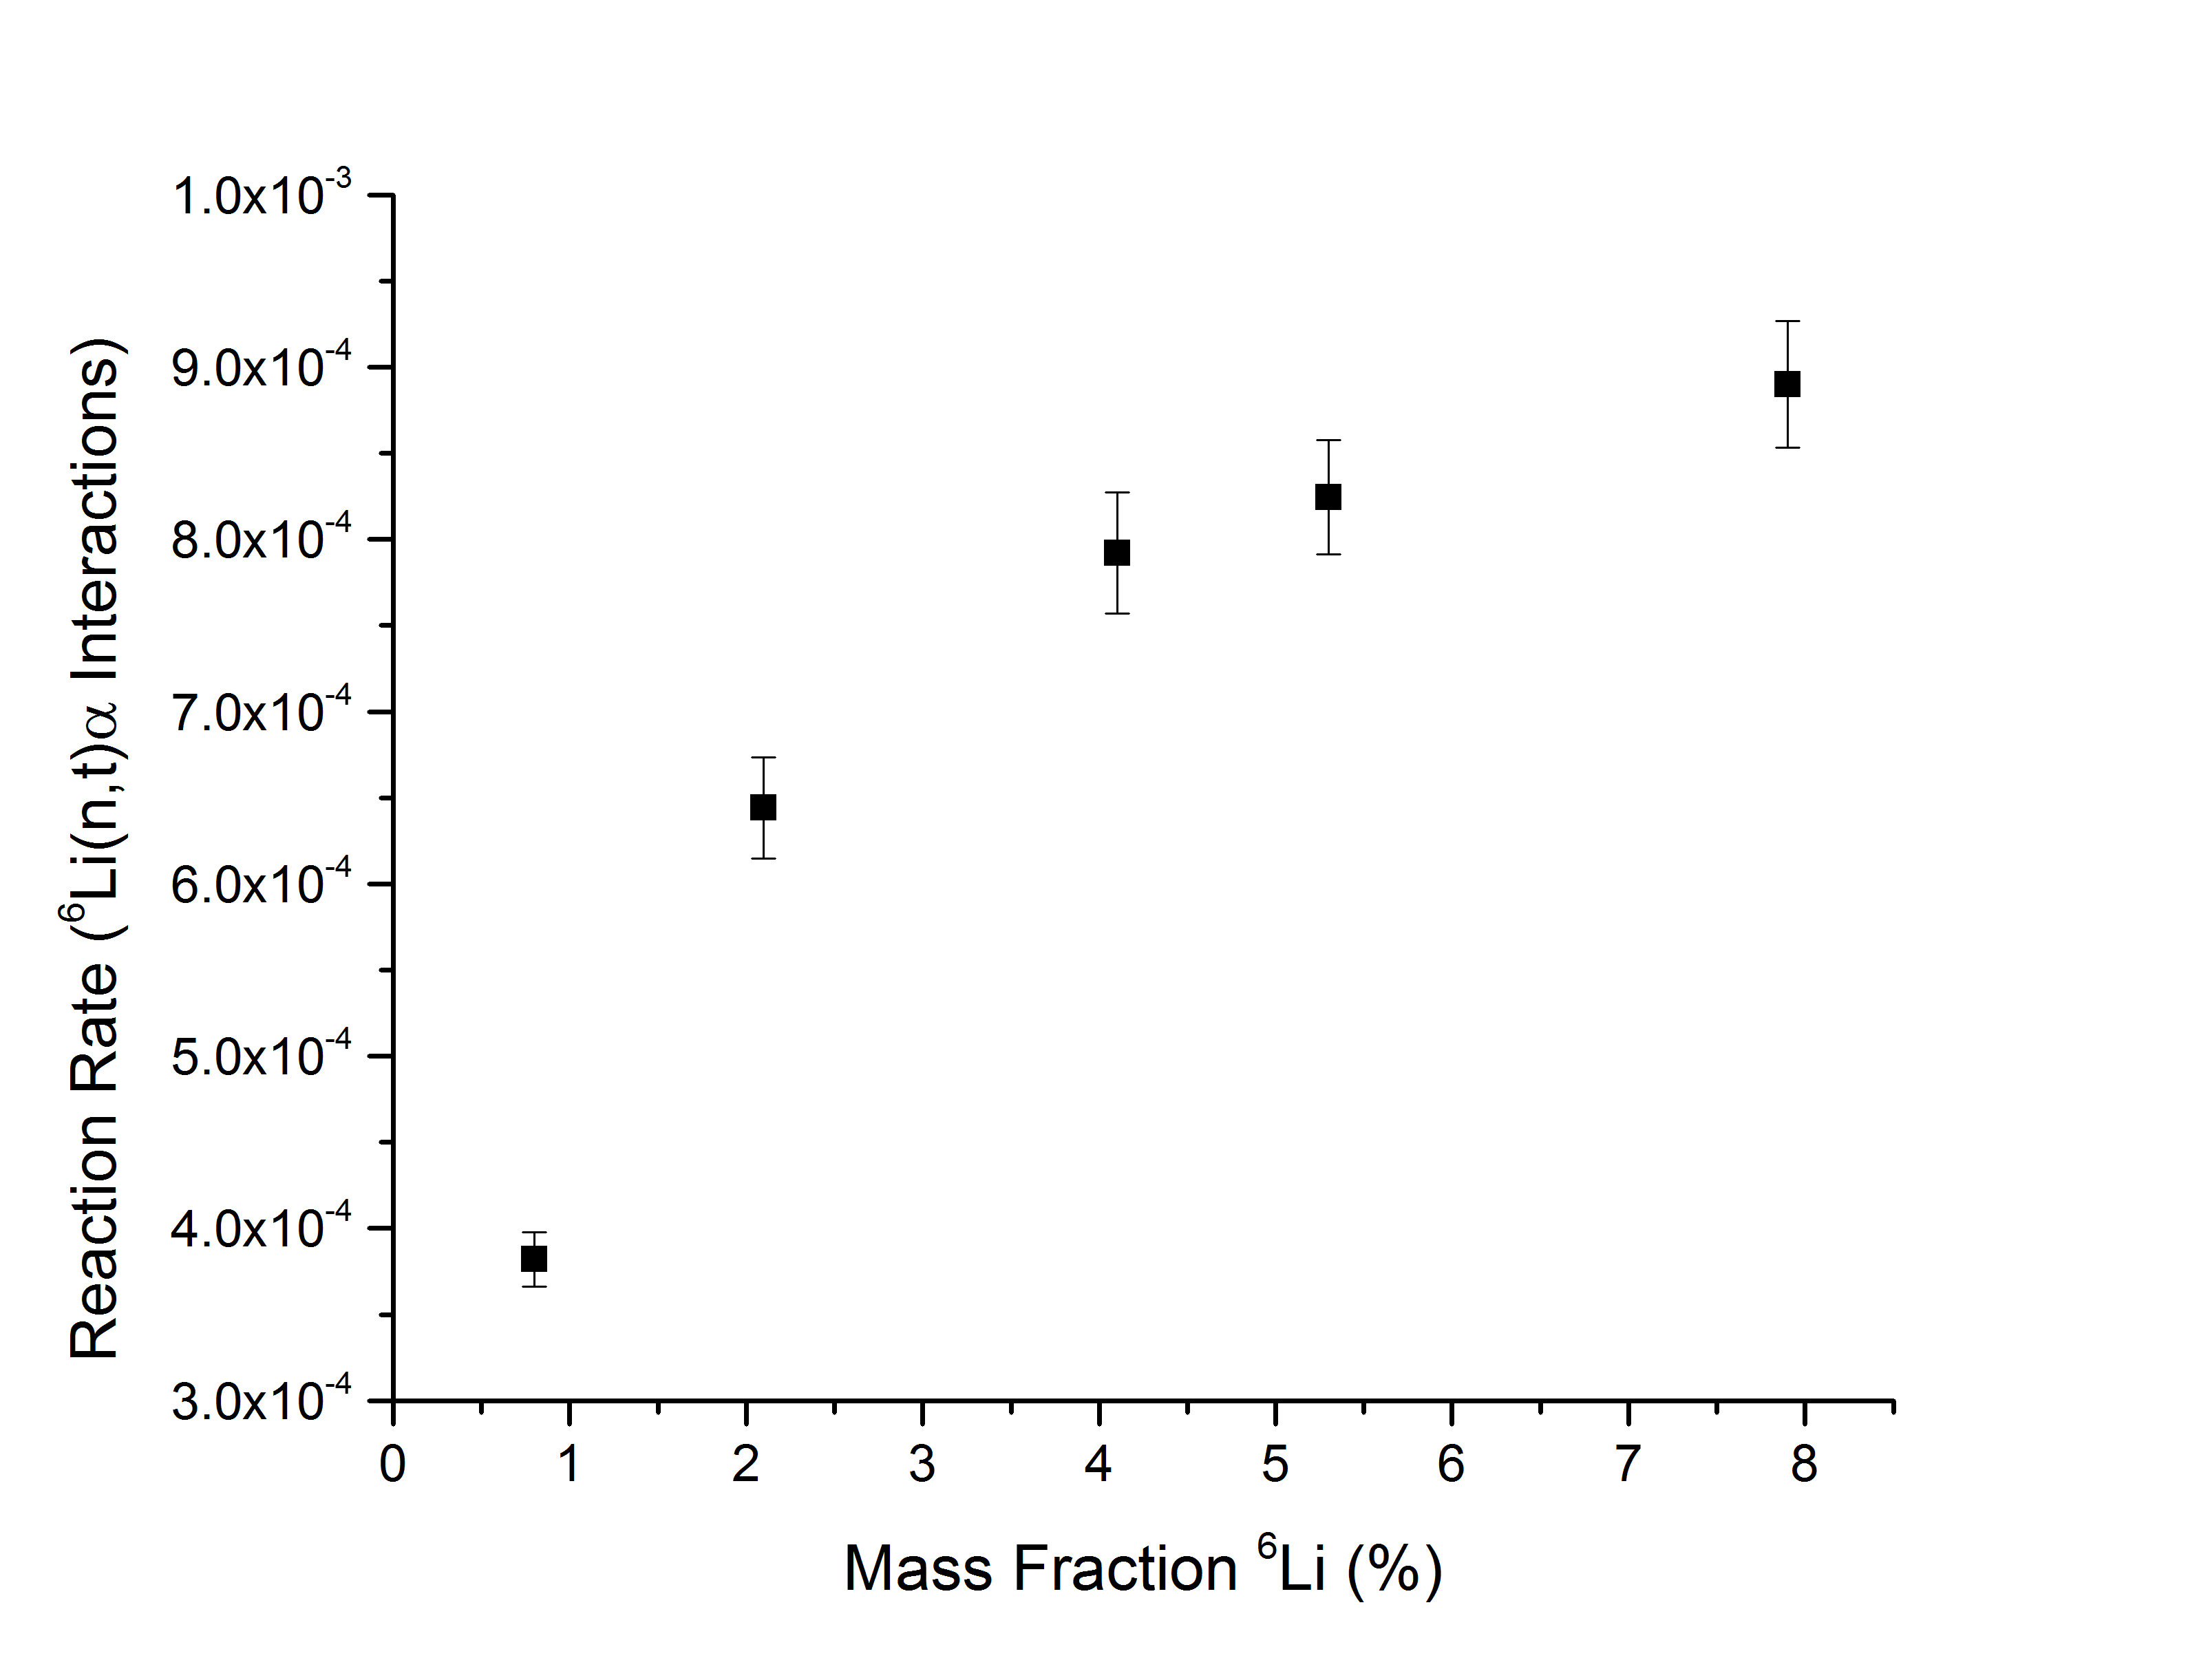
\includegraphics[width=\textwidth]{GS20SelfSheildTotal}
	\caption[Total Reaction Rate]{}
	\label{fig:TotalRxn}
\end{figure}
\end{document}
